\documentclass[aps,prl,twocolumn]{revtex4-1}
\usepackage{graphics,color,graphicx,amsmath}
\usepackage{xr,natbib}
\bibliographystyle{vancouver}
\usepackage{amsbsy}

\newcommand{\norm}[1]{\left\Vert#1\right\Vert}
\newcommand{\abs}[1]{\left\vert#1\right\vert}
\newcommand{\set}[1]{\left\{#1\right\}}
\newcommand{\Real}{\mathbb R}
\newcommand{\eps}{\varepsilon}
\newcommand{\To}{\longrightarrow}
\newcommand{\BX}{\mathbf{B}(X)}
\bibliographystyle{unsrt}
\graphicspath{{images}}

\begin{document}

% COMMANDS -------------------------------------------------------
\newcommand{\mr}[1]{\mathrm{#1}}
\newcommand{\mb}[1]{\mathbf{#1}}
\newcommand{\br}[1]{\left<#1\right>}
\newcommand{\bl}[1]{\left|#1\right|}
\newcommand{\mc}[1]{\mathcal{#1}}
\newcommand{\tb}[1]{\textcolor{blue}{#1}}
\newcommand{\tr}[1]{\textcolor{red}{#1}}
\newcommand{\tg}[1]{\textcolor{green}{#1}}
\newcommand{\si}[0]{\sigma_{\rm i}}
\newcommand{\sj}[0]{\sigma_{\rm j}}
\newcommand{\bs}[1]{\boldsymbol{#1}}

\title{Convenient Interface to Inverse Ising (CONIII): A Python package for solving maximum entropy models}
\author{$^1$Edward D Lee, $^2$Bryan C Daniels}
\affiliation{$^1$Department of Physics, 132A Clark Hall, Cornell University, Ithaca NY 14850, $^2$ASU--SFI Center for Biosocial Complex Systems, Arizona State University, Tempe, AZ 85287}
%\date{}                                           % Activate to display a given date or no date

\begin{abstract}
CONIII is an open-source Python project for providing a simple interface to solving maximum entropy models with a focus on the Ising model. We describe the maximum entropy problem and give an overview of the algorithms that are implemented as part of CONIII (\url{https://github.com/bcdaniels/coniii}) including a regularized mean field method, Monte Carlo histogram, pseudolikelihood, and minimum probability flow. We explain how one should approach and validate maxent models from the perspective of model selection.
%We then show examples of models that have been solved on various data sets using CONIII.
\end{abstract}

\maketitle

\section{Introduction}
Many biological and social systems are characterized by collective behavior whether it is the correlated pattern of neuron firing \cite{Schneidman:2006he}, protein diversity in the immune system, conflict participation in monkeys, flocking in birds \cite{Bialek:2012cs}, statistics of letters in words, or consensus voting in the US Supreme Court \cite{Lee:2015ev}. Statistical physics is a natural approach to probing such systems precisely because they are collective \cite{Castellano:2009ce}.
Recently, with the advent of numerical, analytic, and computation tools, it has become possible to solve for the statistical physics model that corresponds to a particular system, an approach known as the inverse problem.
This is in contrast with the typical problem in statistical physics where one postulates the Hamiltonian and works out the physical behavior of the system. In the \textit{inverse} problem, we  find the parameters that correspond to observed behavior of a known system. In many cases, this is a very difficult problem to solve and does not have an analytical solution, and we must rely on analytic approximation and numerical techniques to estimate the parameters.

The Ising model has been of particular interest because of its simplicity and generality. A variety of algorithms have been proposed to solve the inverse Ising problem, but different approaches are disparately available on separate code bases in different coding languages, which makes comparison difficult and pedagogy more complicated.
CONIII (Convenient Interface to Inverse Ising) is a Python project intended to provide a centralized resource for the inverse Ising problem and provide a base for the addition of more maximum entropy problems in the future. With CONIII, it is possible to solve the inverse Ising problem with a variety of algorithms in just a few lines of code.
%The modular structure of CONIII was inspired by the machine learning package scikit-learn, where each algorithm is implemented in a class.
%There are a variety of techniques for approaching the inverse problem|often in context of a particular model|but they are often presented as different approaches without clear relations to one another. Instead of focusing on the details of each technique separately, we relate these techniques to one another and point out when one would fail or be difficult to apply.

%We hope to provide a (soft) introduction to the analytic, numerical, and computational techniques used to solve these problems to make them accessible to students especially at the graduate level in physics and beyond (and even advanced undergraduates). With the goal of furthering general understanding, we aim not to be rigorous but to be accurate and comprehensible, pointing to the relevant literature whenever possible. Although we strive to be as clear and explicit as possible across this guide, a good background in mathematics or physics will be extremely helpful. In some places, we have left out steps in the derivations, and we encourage the reader to work out the missing steps.

\section{What is maximum entropy?}
Shannon introduced the concept of information entropy in his seminal paper about communication over a noisy channel \cite{Shannon:1948wk}. Information entropy is the unique measure of uncertainty that follows from insisting on some elementary principles of consistency. According to Shannon, information entropy, hereon just ``entropy,'' over the probability distribution of possible discrete configurations $s$ of a system is
\begin{align}
	S[p] &= -\sum_{{\rm s}\in \mathcal{S}} p({\rm s}) \log p({\rm s})
\end{align}
These configurations could be firing on-off patterns in neurons, a the arrangement of 4 letters in a word, or the orientation of spins in a material.

When there is no structure or asymmetry in the distribution|meaning that the probability is uniform $p_s = p_{s'}$|entropy is at a maximum. In the context of communication theory as Shannon first discussed, this means that there is no structure to exploit to make a prediction about the next part of an incoming message; thus, maximum entropy means that each new part of the message is maximally ``surprising.'' In the context of modeling, we use entropy not to refer to the difficulty of the message, but to our state of knowledge about it. When we are uncertain as to the content of the message, we should be precise about our uncertainty.

The idea behind the maximum entropy, or maxent, approach is to build a model that is consistent with the data but otherwise as structureless as possible \cite{Bretthorst:2003ua,Jaynes:1957fy}.
Using entropy as the measure of uncertainty, the formal notion is that we have a constrained maximization problem. From the data, we choose constraints indexed by $k$,
\begin{align}
	\br{f_k(s)}_{\rm data} &= \sum_{s\in \mathcal{S}} p_{\rm data}({\rm s}) f_k({\rm s})
\end{align}

With $K$ constraints, the maximum entropy problem can be solved by the method of Langrangian multipliers. We construct the Langrangian functional $\mathcal{L}$ by introducing the Langrangian multipliers $\lambda_{\rm k}$.
\begin{align}
	\mathcal{L}[p] &= -\sum_s p_s\log p_s - \sum_k^K \lambda_k \left[\br{f_k(s)}-\br{f_k(s)}_{\rm data}\right]\label{eq:Lagrang}
\end{align}
In the notation of statistical physics, the Langrangian is the Helmholtz free energy describing the competition between entropy and the structure described in the Hamiltonian $E$ in equilibrium (See Appendix) \footnote{If we fix the average energy of the system, we get the microcanonical ensemble (See Appendix). which is equivalent to the axiom that all microstates have equal probability (that is the maxent distribution).}.
\begin{align}
	F &= S - \br{E}\\
	E &= -\sum_{\rm k}^K\lambda_{\rm k}f_{\rm k}(s)
\end{align}
This formulation makes clear the fundamental connection that statistical mechanics is an inference procedure using the maximum entropy principle \cite{Jaynes:1957fy}.
Of course, the standard procedure is to  solve for the fixed point by taking the derivative with respect to $\lambda_{\rm k}$.

The resulting model is a Boltzmann distribution over states
\begin{align}
	p(s) &= \left.e^{-E(s)}\right/Z\\
\intertext{with normalization, the partition function,}
	Z &= \sum_{\rm s} e^{-E(s)}
\end{align}

Finding the parameters that match the constraints is equivalent to minimizing the Kullback-Leibler divergence between the model and the data \cite{Cover:2006tl}
\begin{align}
	D_{KL}(p_{\rm data}||p_{\rm ME}) &= \sum_s p_{\rm data} \log\left(\frac{p_{\rm data}(s)}{p_{\rm ME}(s)}\right)\\
	\frac{\partial D}{\partial \lambda_k} &= \sum_s p_{\rm data}(s) \frac{\partial (-E-\log Z)}{\partial \lambda_k}\label{eq:dkl deriv}\\
	0 &= \br{f_k}_{\rm data} -\br{f_k}_{\rm ME}\label{eq:fk-fk}
\end{align}
[Of course, we also have to show that the problem is convex.] In other words, the parameters of the maximum entropy model are the ones that minimize the information theoretic ``distance'' to the distribution of the data. Note that these parameters are given by the data and so there is no search for the best parameters in the conventional sense.

\subsection{Ising model}
The Ising model is a statistical physics model of magnetism \cite{Ising:1924vf}. It consists of a set of spins $\sigma_{\rm i}$ with 2 possible orientations (up and down), each coupled to an external magnetic field $h_{\rm i}$ and coupled to each other with couplings $J_{\rm ij}$. The strength of the magnetic field determines the tendency of each of the spins to orient in a particular direction and the couplings $J_{\rm ij}$ determine whether the spins tend to point together ($J_{\rm ij}>0$) or against each other ($J_{\rm ij}<0$). Typically, neighbors are defined as spins that interact with one another given by some underlying lattice structure as in Figure \ref{gr:ising}.

\begin{figure}[tbp]\centering
	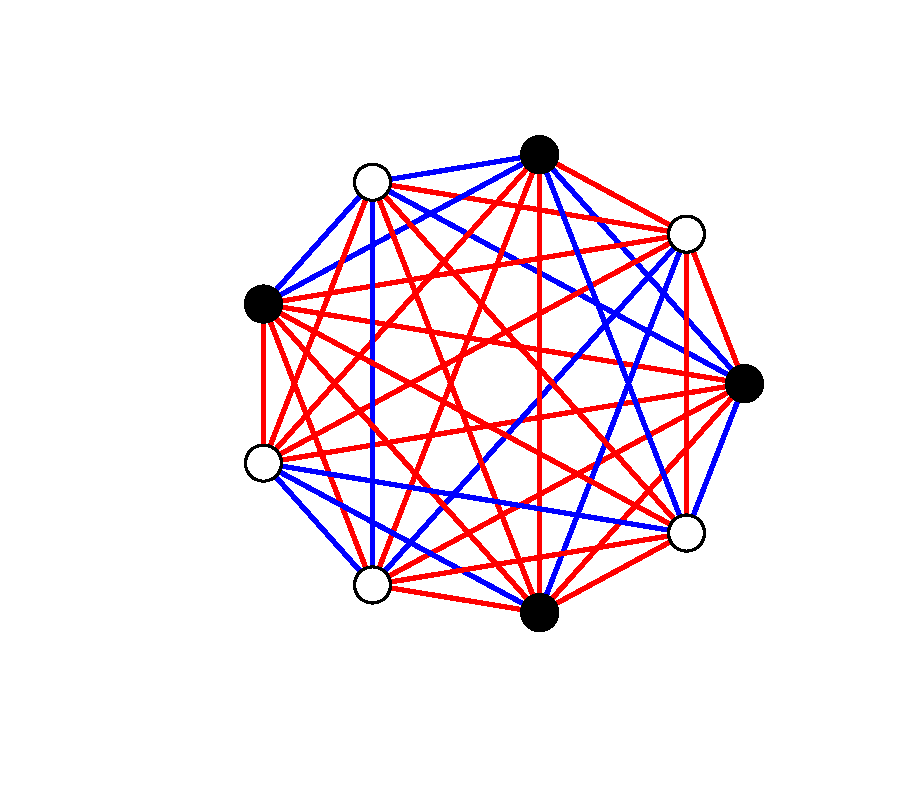
\includegraphics[width=.85\linewidth,clip,trim={100 70 70 60}]{images/ising_example}
\caption{Example of a fully connected Ising model with random couplings.}
\label{gr:ising}
\end{figure}

The energy, or Hamiltonian, of each configuration determines its probability.
\begin{align}
	E &= -\sum_{\rm \br{ij}} J_{\rm ij}\si\sj -\sum_{\rm i=1}^Nh_{\rm i}\si
\end{align}
%States with lower energy are more likely so spin tend to orient along the direction of the local field $h_{\rm i}^{\rm local} = \sum_{\rm j}J_{\rm ij}\sj +h_{\rm i}$. 

We can derive the Ising model from the perspective maximum entropy. Fixing the the means and pairwise correlations to those observed in the data
\begin{align}
	\br{\si}_{\rm data} &= \br{\si}\\
	\br{\si\sj}_{\rm data} &= \br{\si\sj}
\end{align}
we go through the procedure of constructing the Langrangian from Eq~\ref{eq:Lagrang}
\begin{align}
	\mathcal{L}[p] &= -\sum_s p(s)\log p(s) +\sum_{\rm \br{ij}} J_{\rm ij}\br{\si\sj} +\sum_{\rm i=1}^Nh_{\rm i}\br{\si}\\
	\frac{\partial\mathcal{L}[p]}{\partial p(s)} &= -\log p(s)-1 +\sum_{\rm \br{ij}} J_{\rm ij}\si\sj +\sum_{\rm i=1}^Nh_{\rm i}\si\\
	\log p(s) &= -1 +\sum_{\rm \br{ij}} J_{\rm ij}\si\sj +\sum_{\rm i=1}^Nh_{\rm i}\si\\
	p(s) &= \left.e^{-E(s)}\right/Z\\
\intertext{where to enforce normalization of the probability distribution $\sum_s p(s) = 1$,}
	Z &= \sum_s e^{-E(s)}
\end{align}
Thus, the resulting model is exactly the Ising model mentioned earlier.

Despite the simplicity of the Ising model, the structure imposed by the discrete nature of the spins means that finding the parameters is challenging analytically and computationally. In the last few years, numerous techniques have been suggested for solving the inverse Ising problem exactly or approximately \cite{Nguyen:2017ww}. We have made a few of them part of our Python package CONIII to provide a convenient interface for using algorithms already part of the package or adding new algorithms. Here, we briefly describe the algorithms that are part of the first official version of the package. The goal is to give the user a sense (or reminder) of how they work without bogging him or her down in heavy detail. For more detail, we suggest perusing the papers referenced in each section or the review \cite{Nguyen:2017ww}. For a complete beginner, it may be useful to first get familiar with a slower introduction like in the Appendix of Ref \cite{Lee:2015ev}, \cite{Bialek:2012ueb}, or \cite{Jaynes:Logic}.

%Imagine that you have a system with $n$ components that have been sampled many times. To be more specific, we'll take $n=9$ voters on the US Supreme Court that either vote with in the majority, the winning coalition, or in the minority. [More generally, we could think some like gene expression levels in a cell a coarse-grained representation where relatively high or low expression can be represented by a binary variable. Of course, we don't have to restrict ourselves to binary variables \cite{Lezon:2006ws}.]
%The primary difficulty for solving probabilistic models is calculating the normalization because of the size of the state space. Most of the methods below involve avoiding that problem in the first place (Monte Carlo sampling, MCH) or approximations to drastically reduce the state space (pseudolikelihood, adaptive cluster expansion).


\section{Enumeration}
The na\"{i}ve approach that only works for small systems is to write out the equations from Eq~\ref{eq:fk-fk} and solve them numerically. After writing out all $K$ equations,
\begin{align}
	\br{f_{\rm k}}_{\rm data} &= \br{f_{\rm k}}\\
	\br{f_{\rm k}}_{\rm data} &= -\frac{\partial \ln Z}{\partial \lambda_{\rm k}},
\end{align}
we can use any standard optimization algorithm to find the parameters $\lambda_{\rm k}$. 
This approach, however, involves enumerating all terms in the partition function $Z$ whose number grows exponentially with system size. 
%[Simple example with logical gates?]

For the Ising model, the first step in the algorithm for writing down the equations is $\mathcal{O}(K^2 2^{N})$ where $K$ is the number of constraints and $N$ the number of spins. In the second step, each evaluation of the objective in the minimization algorithm will be of the same order. For relatively small systems $n\leq15$, however, this approach is feasible on a typical desktop computer and is a good way to test the results of a more complicated algorithm.

This approach is part of the {\tt Exact} class that contains code for writing Eqs~\ref{eq:fk-fk} into a file and solving them with the {\tt scipy.optimize} library.


\section{Monte Carlo method}
Perhaps the most straightforward and most expensive computational approach is to use Monte Carlo Markov Chain (MCMC) sampling to approximate the distribution and adjust the parameters appropriately after each step. The parameters are adjusted using a learning rule, and both sampling and learning is repeated til the stopping criterion is met.
The magic behind MCMC approaches is that only relative probabilities of states need to be known to return a sample of the distribution. Thus, we do not need to calculate the partition function, but can instead compute the difference in energy between two states. This can be combined with a variety of stochastic gradient descent methods to reduce the number of sampling steps. The particular technique implemented in CONIII is the Monte Carlo Histogram method \cite{Broderick:2007wq}.

Since the sampling step is expensive, the idea behind Monte Carlo histogram is to reuse a sample for more than one gradient descent step because we can predict how the distribution will change if we modify the parameters slightly \cite{Broderick:2007wq}. Given that we have a sample with probability distribution $p_s$ generated with parameters $\lambda_{\rm k}$, we would like to estimate the new distribution $p_s'$ from adjusting our parameters $\lambda_{\rm k}' = \lambda_{\rm k}+\Delta\lambda_{\rm k}$. We can leverage our current sample to make this extrapolation.
\begin{align}
	p_s' &= \frac{p'_s}{p_s}p_s\\
		&= \frac{Z}{Z'}e^{\sum_k \Delta\lambda_k f_k(s)} p_s\\
\intertext{To estimate the average,}
	\sum_s p_s' f_k(s) &= \frac{Z}{Z'} \sum_s p_s e^{\sum_k \Delta\lambda_k f_k(s)} f_k(s)\\
\intertext{To be explicit about the fact that we only have a sampled approximation to $p$,}
	\br{f_k}' &= \frac{Z}{Z'} \br{e^{\sum_k \Delta\lambda_k f_k(s)} f_k(s)}_{\rm sample}
\end{align}
Likewise, the ratio of the partition function can be estimated
\begin{align}
	\frac{Z}{Z'} \approx 1\left/\br{e^{\sum_k \Delta\lambda_k f_k(s)}}_{\rm sample}\right.
\end{align}

The main difficulty with MCH is choosing a learning rule for how to update the Lagrangian multipliers $\{\lambda_k\}$ at each iteration while being careful to stay within the bounds of a reasonable extrapolation. One suggestion is to update the parameters with some inertia
\begin{align}
	\Delta\lambda_k(t+1) &= \Delta \lambda_k(t) + \eta \Delta\lambda_k(t-1)\label{eq:mch learn1}\\
	\Delta \lambda_k(t) &= \epsilon\left(\br{f_k}'-\br{f_k}\right)\label{eq:mch learn2}
\end{align}
This has the correct fixed points. One suggestion is to shrink $\epsilon$ exponentially with the number of iterations. 
%Another heuristic is to begin with a small sample size and increase the size of the sample set as we refine our estimates of the parameters.

In practice, MCH can be difficult to tune properly and one must check in on the progress of the algorithm often. One issue is that parameters cannot be changed by too much or the extrapolation to $\lambda_{\rm k}'$ will be inaccurate and the algorithm will fail to converge. In CONIII, this can be controlled by setting a bound on the maximum possible change in each parameter  $\Delta\lambda_{\rm max}$ and restricting the norm of the vector of change in parameters $\sum_k \sqrt{\Delta\lambda_{\rm k}^2}$. Another issue is setting the parameters of the MCMC sampling routine. Both the burn time (the number of iterations before starting to sample) and sampling iterations (number of iterations between samples) must be large enough that we are sampling from the equilibrium distribution.  Typically, these are found by looking at the decorrelation time in the energy or correlations as a function of MCMC iterations made. The parameter may need to be updated during the course of MCH because the sampling parameters may need to change with the estimated parameters of the model. To add further complications, for some sets of parameters samples are correlated over long times and alternative sampling methods must be used.
We do not discuss these sampling details here, but see Ref \cite{MacKay:2005wc} for examples.

The main computation cost for MCH is the sampling step. The runtime is proportional to the number of samples $n_{\rm sample}$, number of MCMC iterations $n_{MC}$, the number of constraints $K$:
$\mathcal{O}(n_{\rm MC} n_{\rm sample} K)$, whereas the MCH estimate is relatively quick $\mathcal{O}(n_{\rm sample}n_{\rm MCH}K)$ because the number of MCH approximation steps is much smaller than the number of MCMC sampling iterations $n_{\rm MCH}<<n_{\rm MC}$. 
%What is the runtime for the learning rules Eqs \ref{eq:mch learn1} and \ref{eq:mch learn2}?
For the Ising model, $K\sim N^2$, the system size squared.

MCH is implemented in the {\tt MCH} class.

\section{Pseudolikelihood}
The pseudolikelihood approach is an analytic approximation to the likelihood that drastically reduces the computational complexity of the problem and is exact in the thermodynamic limit \cite{Aurell:2012hi}. We maximize the conditional probability of each spin $s_{\rm i}$ given the rest of the system
\begin{align}
	p\left(s_{\rm i}|{\bf s}_{\backslash \rm i}\right) &= \left( 1+e^{-2s_{\rm i} \left(h_{\rm i}+\sum_{j\neq i}J_{\rm ij}s_{\rm j}\right)} \right)^{-1}
\end{align}
Taking the logarithm and summing over all spins, we define the approximate likelihood to be summed over all data points indexed by $r$.
\begin{align}
	f(h_{\rm i},\bs{J}_{\rm i}) &= \sum_{\rm r=1}^R \ln p\left(\left.s_{\rm i}^{(r)}\right|\bs{s}_{\backslash\rm i}^{(r)}\right)
\end{align}
In the limit where the ensemble is well sampled, the average over the data can be replaced by an average over the ensemble
\begin{align}
	f(h_{\rm i},\bs{J}_{\rm i}) &= \sum_{\bs{s}} \ln p\left(\left.s_{\rm i}^{(r)}\right|\bs{s}_{\backslash\rm i}^{(r)}\right)p(\bs{s};h,J)\\
\intertext{At maximum likelihood,}
	\frac{\partial f}{\partial J_{\rm ij}} &= \sum_{\bs{s}} \ln p\left(\left.s_{\rm i}^{(r)}\right|\bs{s}_{\backslash\rm i}^{(r)}\right)p(\bs{s};h,J)\\
	0 &=
\end{align}

Pseudolikelihood is extremely fast. Each iteration only is $O(RN^2)$ and often surprisingly accurate.

We have implemented pseudolikelihood for the Ising model in {\tt Pseudo}.

\section{Minimum Probability Flow}
Minimum probability flow involves analytically approximating how the probability distribution \textit{changes} as we modify the \textit{configurations} \cite{SohlDickstein:2011im}. In the methods so far mentioned, the approach has been to maximize the objective (the likelihood function) by immediately taking the derivative with respect to the parameters. With MPF, we first posit a set of dynamics that will lead the data distribution to equilibrate to that of the model. When these distributions are equivalent, then there is no ``probability flow'' between them. This technique is closely related to score matching where instead we have continuous state spaces and can directly take the derivative with respect to the states without specifying dynamics \cite{Hyvarinen:2007ed}.

As before, we start with minimizing the Kullback-Leibler divergence, but instead of taking the derivative with respect to the parameters, we first ask how the probability flows between the model and the states in the data $\mathcal{D}$ if the dynamics are run for an infinitesimal amount of time $\epsilon$, the idea being that the relative difference between the probability distributions are minimized with optimal parameters.
\begin{align}
	\partial_t D_{KL}(p^{(0)}||p^{(t)}\left(\{\lambda_k\}\right)) &= \sum_{\rm s \not\in \mathcal{D}} \dot{p}_{\rm s}(\lambda_k)\\
	K(\{\lambda_{\rm k}\}) &= \sum_{\rm s \not\in \mathcal{D}} \dot{p}_{\rm s}(\lambda_k)
\end{align}

Monte Carlo dynamics (satisfying ergodicity and detailed balance) would lead to equilibration of the two distributions. A simple transition matrix suggested in Ref \cite{SohlDickstein:2011im} is
\begin{align}
	\dot{p}_{\rm s} &= \sum_{s'\neq s} \Gamma_{\rm ss'} p_{\rm s'} -\sum_{\rm s'\neq s} \Gamma_{\rm s's} p_{\rm s}\\
	\Gamma_{\rm ss'} &= g_{\rm ss'}\exp\left[ \frac{1}{2}\left( E_{\rm s'}-E_{\rm s} \right) \right]
\end{align}
with transition probabilities $\Gamma_{\rm ss'}$ from state ${\rm s'}$ to state s. The connectivity matrix $g_{\rm ss'}$ specifies whether there is edge between states s and ${\rm s'}$ such that probability can flow between them. By choosing a sparse $g_{\rm ss'}$ while not breaking ergodicity, we drastically reduce the computational cost of calculating the objective function.

Finally, we must find the minimum of the objective function
\begin{align}
	K(\{\lambda_{\rm k}\}) &= \sum_{\rm s \not\in \mathcal{D}} \dot{p}_{\rm s}(\lambda_k)
\end{align}

MPF satisfies a number of useful properties:

At each step of the algorithm for the Ising model, the runtime is $O(RN^2)$.

MPF is implemented in the {\tt MPF} class.


\section{Regularization to avoid overfitting}

Besides the computational complexity of locating best-fit parameters,
a fundamental problem in any model inference method is that uncertainty coming
from the finiteness of data translates into uncertainties in parameters.
The straightforward answer to this problem is to take more data---in a pairwise
maximum entropy problem, we might insist that we have enough samples to well-constrain
the correlation between every pair of individuals.  But it is not always possible
to take enough data.  For instance, in a social system in which we are trying to
measure stable social structure that lasts on the order of months, there are only
a finite number of social interactions that occur over those months, which may
not be enough to tightly constrain parameters.

The danger in naively searching for a best-fit solution in a data-poor situation
is overfitting, or erroneously finding patterns in the finite-sample noise.
One way to avoid overfitting is regularization:
restricting the search space in some principled way so that more complicated
solutions are disallowed.  We then check that the regularized solutions fit the
data within expected statistical fluctuations.  If not, a more lax regularization
can be used to allow more complicated solutions that are able to fit the
remaining signal in the data.

We will motivate the next two approaches to maximum entropy fitting in terms
of regularization.

[This section might be tightened a bit more.  For one, I am somewhat confused as
to whether the entire maximum entropy approach might be motivated in this
way---starting with few constraints and adding the possibility of higher order
constraints until the model fits well enough.]


\section{Mean-field method}
One attractively simple and efficient version of the regularized approach starts
with mean-field theory.  In the inverse Ising problem, mean-field theory is equivalent
to treating each binary individual as instead having a continuously varying state
(corresponding to its mean value).  The inverse problem then turns into simply inverting
the correlation matrix $C$: \cite{CocMon12}
\begin{equation}
\label{meanFieldSolution}
J^{\mathrm{mean-field}}_{k\ell} =
    - \frac{ (C^{-1})_{k\ell} }{ \sqrt{p_k(1-p_k)p_\ell(1-p_\ell)} },
\end{equation}
where
\begin{equation}
C_{k\ell} = \frac{ p_{k\ell} - p_k p_\ell }{ \sqrt{p_k(1-p_k)p_\ell(1-p_\ell)} },
\end{equation}
and where $p_k$ corresponds to the frequency of individual $k$ being
in the active ($+1$) state and $p_{k\ell}$ is the frequency of the pair
$k$ and $\ell$ being simultanously in the active state.

A simple regularization scheme in this case is to discourage large values in the interaction
matrix $J$.  This corresponds to putting more weight on solutions that are closer to
the case with no interactions (independent individuals).  A particularly convenient form
adds the following term, quadratic in $J$, to the negative log-likelihood:
\begin{equation}
\gamma \sum_i \sum_{j > i} J_{ij}^2 p_i (1-p_i) p_j (1-p_j).
\end{equation}
In this case, the regularized version of the mean-field solution in \eqref{meanFieldSolution}
can be solved analytically, with the slowest computational step coming from the inversion
of the correlation matrix.  For details, see Refs.~\cite{DanKraFla17,BarCoc13}.

The idea is then to vary the regularization strength $\gamma$ to move between the
non-interacting case ($\gamma \rightarrow \infty$) and the naively calculated
mean-field solution \eqref{meanFieldSolution} ($\gamma \rightarrow 0$).
While there is no guarantee that varying this one parameter will produce solutions that are
good enough to ``fit within error bars,'' this approach has been successful in at least
one case of fitting social interactions \cite{DanKraFla17}.

This is implemented in {\tt RegularizedMeanField}.



\section{Cluster expansions}

Adaptive cluster expansion \cite{CocMon11,CocMon12,BarCoc13}
iteratively calculates terms in the
cluster expansion of the entropy $S$:
\begin{equation}
S = \sum_\Gamma \Delta S_\Gamma,
\end{equation}
where the sum is over clusters $\Gamma$ and in the exact case
includes all $2^N - 1$ possible nonempty subsets of individuals in the system.
\footnote{In the simplest version of the expansion,
one expands around $S=0$.  In some cases it can be more advantageous to write the
expansion around $S-S_0$, where $S_0$ is a reference entropy corresponding to
an easily calculated case such as
the independent individual solution or one of the mean-field solutions
described in the previous section \cite{BarCoc13}.}
The inverse Ising problem is solved independently
on each of the clusters, which can be done exactly when the
clusters are small.  These results are used to construct a full
interaction matrix $J$.
The expansion starts with small clusters and expands to use larger
clusters, neglecting any clusters whose
contribution $\Delta S_\Gamma$ to the entropy falls below a threshold.
To find the best solution that does not overfit,
the threshold is initially set at a large value and then lowered,
gradually including more clusters in the expansion, until samples from
the resulting $J$ fit the desired statistics of the data sufficiently well.

In Coniii, the selective cluster expansion method is implemented in the {\tt ClusterExpansion} class.

%\section{Bethe/Kikuchi free energy/cavity methods}
%Another approach involves a cluster-expansion of the free energy, also known as the cavity method. This has not yet been implemented in CONIII.
%The cavity method involves use of the marginalized distribution.

\section{Incomplete data}

\section{Samplers}
In CONIII, we have implemented two versions of the Metropolis algorithm. One is specific to the Ising model {\tt MCIsing} and the other {\tt MC} can sample a system as long as the function for calculating the energy is supplied by the user.

In some parameter regimes, where spins are tightly correlated, the Metropolis algorithm is very inefficient. Cluster sampling like Wolff or Swendsen-Wang are much more efficient.

%\section{Algorithm for solving}
%We suggest solving the inverse problem using a fast technique. 
\section{Discussion}
\subsection{Validation}
The first step in validating a maxent model is to confirm that it matches the given constraints.  In the cases where we use an approximate technique or regularize the problem, we must make sure that it matches the data within reasonable error bars given by the data. Assuming that the data is independently and identically distributed, the errors are given by the standard error of the mean of a binomial distribution \mbox{$p_{\rm ij...k} = p(s_{\rm i}=s_{\rm j}=...=s_{\rm k}=1)$} with $K$ data points.
\begin{align}
	\delta_{\rm ij...k} &= \sqrt{(1-p_{\rm ij...k})p_{\rm ij...k}/K}
\end{align}

Since the model is only fit to the given constraints, it is not given that it will be able to fit other features of the data that have not been specified. For the Ising model, a good fit to any higher order feature of the probability distribution is in this sense nontrivial. 

Basic checks would be to compare against higher order correlations in the data. In Figure~??, we show an example of a pairwise maxent model tested against higher order correlations. Since these are quantities averaged over the joint probability distribution of many spins, a stricter check would be to compare the entire probability distribution of the pairwise maxent model with that of the data \cite{Lee:2015ev}, but this is only feasible when the data set is reasonably large. For each problem, there are specific features that are more relevant to the question at hand, which would be important to check. For conflict in monkeys, a coarse-grained feature is the distribution of conflict sizes which seems to have a characteristically long tail, and that is checked specifically \cite{Daniels:1cq}. 

\subsection{Model complexity}
How do we know if we need to add more parameters? To answer this question, we need a way of quantifying the tradeoff between the complexity and fit of the model. The idea is that a more complicated model gives us more information about the data set that we are fitting, but specifying the parameters also requires information. This is tradeoff between the information gain and the information cost. Roughly speaking, we can imagine that specifying the $K$ parameters is localizing a region in a high-dimensional space. The volume of the ``ball'' grows like $l^K$, so that the information cost goes like $K\log(l)$. This is the picture formalized by quantities like the Akaike information criterion (AIC) or the Bayesian information criterion (BIC) \cite{}. An accessible description of model selection with maximum entropy is described in Ref \cite{Lee:2015ev}.

Choosing which parameters to impose is an important question. Typically, the approach has been to constrain the lowest order interactions that are sufficient to produce collective behavior. The intuition from physics is from the observation that many physical systems are extremely well (if not exactly) described by pairwise interactions. In statistical physics, the observation that highly correlated behavior across space and time can emerge from pairwise interactions has even stronger justification from renormalization group theory \cite{}. In fact, the ability to model a system well with only pairwise interactions may be surprising \cite{Ranganathan:2007wz}. From the model fitting perspective, however, we might choose to constrain other parts of the probability distribution. In Ref \cite{Schneidman}, they  explore choosing correlations to constrain depending on whether or not they are signicantly large. In Ref \cite{Nemena}, how a pairwise model becomes an increasingly effective description of a system with higher order interactions as the system gets larger.

\subsection{Conclusion}
Science is a process of model selection. In the ideal picture, we start with the simplest models and the fewest constraints possible, and then we increase the complexity of the model til it is sufficiently so to make good predictions. In principle, we could add as many contraints as would allow us to fit the data well, but the idea is that complex models are not only ``expensive'' but they do not generalize well.
Maxent is a principled framework for this picture of model building. The number of parameters and the order of the constraints we impose can be adjusted to test our hypotheses about what matters for the system.
In this sense, the maxent approach is a useful ``model'' framework for thinking about statistical inference problems far beyond statistical physics. We build an open-source Python package that we hope will be accessible and useful for those unfamiliar with maxent approaches to experiment and perhaps apply this technique to their questions.



\clearpage
\appendix

\section{The microcanonical ensemble and maximum entropy}
The conventional textbook in statistical mechanics first introduces the concept of entropy as a way of counting the phase volume available to the system at a given energy
\begin{align}
	S(E) &= k_B \log\Omega(E)
\end{align}
where $k_B$ is Boltzmann's constant and $\Omega$ the number of states between $E$ and $E+\delta E$. Temperature is defined as
\begin{align}
	\frac{1}{T} &= \frac{\partial S}{\partial E}
\end{align}

 begins with the concept of a small system coupled to a heat bath. In this limit, we can linearly expand thermodynamic quantities about the energy of the bath $E_{\rm bath} = E-E_s$
\begin{align}
	S_{\rm bath}(E-E_s) &\approx S_{\rm bath}(E) -E_s\left.\frac{\partial S}{\partial E_s}\right|_{E-E_s}\\
		&= S_{\rm bath}(E) -\frac{E_s}{T}\\
	e^{S_{\rm bath}(E-E_s)/k_B} &= e^{S_{\rm bath}(E)/k_B} e^{-E_s/k_BT}
\intertext{Since the entropy is proportional to the density of states at a particular energy $E_s$, Eq ?? corresponds to}
	p(E_s) &= e^{-E_s/k_BT}/Z
\end{align}
With partition function $Z$. In other words, the Gibbs measure takes exponential form. Eq ?? can be rewritten in terms of free energy
\begin{align}
	\log p(E_s) &= -E_s/k_BT -\log(Z)
\intertext{Averaging both sides over all energy configurations and rearranging}
	-k_B T\log Z &= \sum_s p(E_s) E_s +k_BT\sum_s p(E_s)\log p(E_s)
\intertext{Remembering the fundamental postulate of statistical mechanics that all states are equally likely}
	-k_BT\log Z &= \br{E_s} - TS\\
	F &= \br{E_s} -TS
\end{align}
This equation tells us how the Helmholtz free energy is related to the internal energy and the entropy of the system.

When we say that free energy is minimized for a system with Hamiltonian $E_s$ at equilibrium, we are equivalently saying that entropy is maximized. Entropy maximization is the crux of statistical physics models.
%A more colloquial way of stating this is that statistical mechanics models produce a distribution that is as ``spread out'' as possible given a particular form to the energy function and a temperature.

\section{Notes on Monte Carlo Markov Chain sampling}
The key points behind MCMC sampling is ergodicity and detailed balance. Ergodicity just means that we can get from one state to another in a finite number of steps, and this ensures that we don't get stuck in a few states. Detailed balance is a sufficient but not necessary condition (stronger than needed) for ensuring that the equilibrium distribution matches the distribution that we seek. There are some specialized algorithms that don't satisfy detailed balance but do produce the desired distribution.

To check whether an algorithm works, one must prove that both these conditions are satisfied. Ergodicity is usually trivial. Typically, we write down the condition for detailed balance for any two states $a$ and $b$,
\begin{align}
	p(a|b)p(b) &= p(b|a)p(a) \\
	p(b)/p(a) &= p(b|a)/p(a|b) \\
	e^{-(E_b-E_a)} &= 
\end{align}
A reasonable way to do this would be to take $p(b|a) = e^{-(E_b-E_a)}$ and $p(a|b) = 1$ when $E_b>E_a$.

\begin{align}
	p_a\,T(a\rightarrow b)A(a\rightarrow b) &= p_b\,T(b\rightarrow a)A(b\rightarrow a)\\
	p_a/p_b &= T(b\rightarrow a)A(b\rightarrow a)/T(a\rightarrow b)A(a\rightarrow b)
\end{align}
where $T$ is the transition probability and $A$ is the acceptance probability. For a Boltzmann type model, this means that this ratio must be equal to $\exp(-\beta(E_a-E_b))$.

\subsection{Swendsen-Wang}
As an example, we consider the Swendsen-Wang cluster algorithm. In this algorithm, the first step is to form bonds between like spins (to grow clusters) then we flip to any configuration permitted by the current bond structure which is uniform. If you work through the calculations (GNB V pg 81), you will find that the probability of transitioning between states depend on the bonds that could have formed between like spins but didn't, and this is equal to the energy difference between the states.

\subsection{Wolff}
Another example is the Wolff algorithm (see GNB V pg 83) which is like the SW algorithm except that only a single cluster is build and flipped at a time with probability 1, i.e. the acceptance probability is 1 in the original algorithm. We start with any random site as the initial spin then we build a cluster spreading out from that spin to its nearest neighbors where the choose the probability of choosing a neighbor to be $1-\exp(-2J_{ij})$.

The random fields can be accounted for in the acceptance probabilities (so the probability of a cluster flipping is no longer 1). Working through the math, you will find that the cluster growth accounts for the ratio of the energies that come from the couplings but to account for the fields, the probability of a particular orientation of the clusters has to be
\begin{align}
	p(\Sigma_n) &\propto \exp\left(\sum_i h_i\sigma_i\right)
\end{align}
which we can easily simulate using something like the Metropolis algorithm. Obviously, this will increase the correlation time between samples because we will not always accept a cluster flip. This can be especially problematic when the clusters become large and have similar fields, but as long as the sum of the distribution of local fields for spins in a cluster is symmetric about 0, this will not be too slow. Certainly, it is faster than any local flip algorithm.

A simple example that I worked through is with 4 spins and the transition probability between two different states. Here, we can easily enumerate all possible ways of transitioning between these two states using the Wolff algorithm.

\section{Replica exchange Monte Carlo (REMC)}
REMC simulates multiple replicas of the system at different temperatures simulaneously and allow states to be exchanged between them. The idea is that an energy barrier may be very difficult to cross below a certain critical temperature, but there may be a trajectory allowed by diffusing through higher temperatures to cross the boundary.

Instead of considering the ensemble of a single system, we consider the ensemble of multiple independent systems. Thus, the joint probability distribution on the extended state space is
\begin{align}
	p(\sigma,\beta_n).
\end{align}
where $\beta_n = 1/T_n$ is the inverse temperature.

The simplest possible assumption for the shape of this distribution would be that the probability of occupying any particular temperature $\beta_n$ is uniform $p(n) = 1/N_T$. It turns out that this is optimal according to some criterion (see citation in Kerler and Rehberg). Note that this is not the same as just simulating a set of replicas for which the partition funtion would be
\begin{align}
	Z &= \prod_{m} \sum_\sigma \exp\left[ -\beta_m H(\sigma) \right] \label{eq:equi Z}
\end{align}
This is for the obvious reason that the average energy is a function of $T$ so a simulation of Eq \ref{eq:equi Z} would spend much more time exploring lower temperatures than higher temperatures. This makes it difficult to have the system use higher energy states to cross energy barriers. 

So instead of Eq \ref{eq:equi Z}, we can include a term $g_n$ to compensate
\begin{align}
	Z &= \prod_{m} \sum_\sigma \exp\left[ -\beta_m H(\sigma) +g_m \right]
\end{align}
How do we find $g_n$?

Under the assumption that the probability $p(n)$ is a constant,
\begin{align}
	p(n) &= e^{g_n} \sum_\sigma \exp\left[ -\beta_n H(\sigma) \right]/Z\\
	g_n &= \log[p(n)\,Z] + \tilde{Z}_n\\
	g_n &\rightarrow \tilde{Z}_n
\end{align}
(remembering that constants don't matter in the relation between energy and probability) where 
\begin{align}
	\tilde{Z}_n &= \sum_\sigma \exp\left[ -\beta_n H(\sigma) \right]
\end{align}
One way to find the $g_n$ that satisfy this condition is to come up with an iterative algorithm that converges to a fixed point. One suggestion is to estimate $g_n$ by reweighting the distributions from adjacent replicas.

Now, it remains to find a set of $\beta_n$ that is optimal for simulating relaxing into equilibrium quickly. One suggestion to make the algorithm spend an equal amount of time at each temperature. Kerler and Rehberg suggest a method.

\bibliography{guide}

\end{document}  
